\pagestyle{fancy}
\fancyhead[LO]{\autorR}
\fancyhead[LE]{\autorA}
\fancyhead[RE,RO]{\textit{\rightmark}}
\fancyfoot[L]{\asignaturaAbbr}
\fancyfoot[R]{\fecha}

\section{Producto matricial en GPU} \label{sec:3}
En esta sección se analiza el rendimiento del producto matricial en GPU. Para ello, se ha implementado un \textit{kernel} 
que realiza el producto de dos matrices de tamaño $N \times N$ y se ha medido el tiempo de ejecución en función del tamaño de 
la matriz. Cada tamaño de matriz se ha ejecutado con todos los bloques de hilos posibles ($1, 2, 4, 8, 16, 32$).

\subsection{CPU vs GPU}
Se compara a continuación el rendimiento del producto matricial en CPU y en GPU. Para ello, se grafican los resultados obtenidos 
con el algoritmo \zorder\ en CPU y con el \textit{kernel} paralelizado en GPU utilizando 1 \textit{thread per block}. Dichos 
resultados se muestran en la \autoref{fig:1}.

\begin{figure}[h]
    \centering
    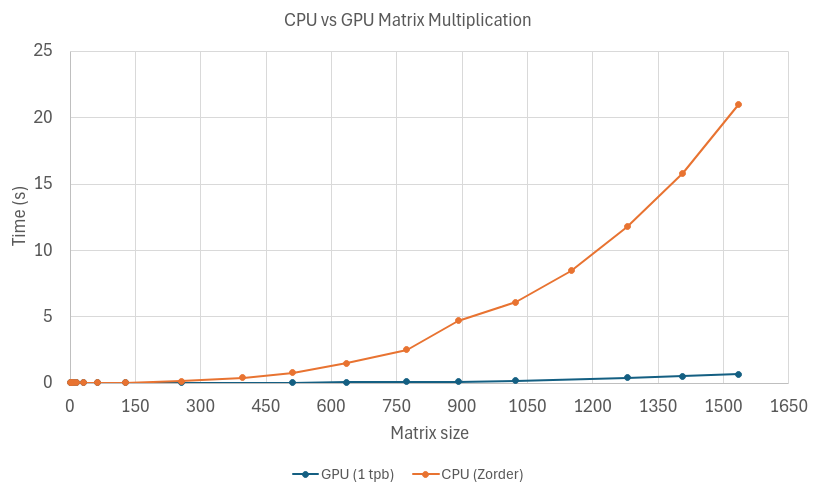
\includegraphics[width=0.5\textwidth]{img/1.png}
    \caption{Rendimiento del producto matricial en CPU y GPU}
    \label{fig:1}
\end{figure}

Como se puede observar, el rendimientro del producto matricial en GPU es infinitamente superior al de CPU. Además, debe tenerse en 
cuenta que se está utilizando el algoritmo probado en CPU que mejores resultados ha dado (\zorder) respecto a la configuración 
menos eficiente en GPU (1 \textit{thread per block}). 

\subsection{\textit{Threads per block}}
En esta sección se analiza el rendimiento del producto matricial en GPU en función de la cantidad de \textit{threads per block}
utilizados. Los resultados se grafican en la \autoref{fig:2}.

\begin{figure}[h]
    \centering
    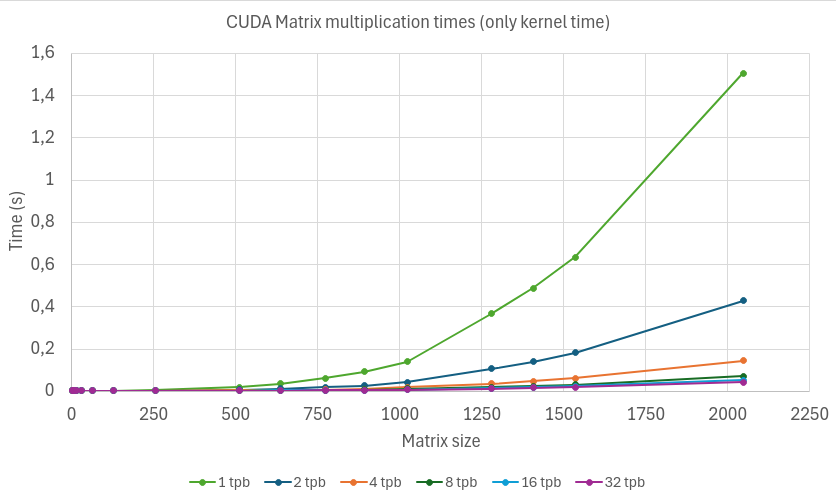
\includegraphics[width=0.5\textwidth]{img/2.png}
    \caption{Rendimiento del producto matricial en GPU en función de los \textit{threads per block}}
    \label{fig:2}
\end{figure}

Como es de esperar, el rendimiento mejora a medida que se incrementa el número de \textit{threads per block}. Esta mejora de rendimiento 
se hace mucho más notable conforme aumenta el tamaño de la matriz, aunque en este caso, a partir de $8$ \textit{threads per block} puede
considerarse despreciable. Esto se debe a que el máximo tamaño de matriz probado ($N=2048$) es relativamente pequeño y no se aprovechan
al máximo las capacidades de la GPU. En la \autoref{fig:3} se observa el rendimiento del producto matricial en GPU con matrices 
mucho mayores.

\begin{figure}[h]
    \centering
    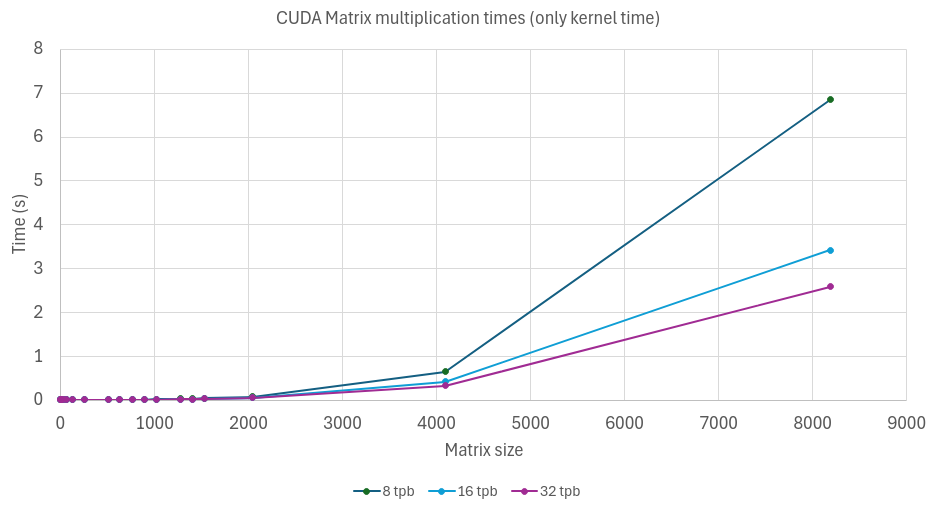
\includegraphics[width=0.55\textwidth]{img/3.png}
    \caption{Rendimiento del producto matricial en GPU con matrices de tamaño $N>2048$}
    \label{fig:3}
\end{figure}

Ahora sí que la diferencia de rendimiento con más de $8$ \textit{threads per block} es notable, y será aun mayor utilizando matrices 
de más tamaño. 

\subsection{Reserva de memoria y copia de resultados}
Una peculiaridad de la GPU es que su memoria no es accesible desde la CPU. Por lo tanto,
es necesario reservar memoria en la GPU para almacenar los resultados y luego copiarlos a la memoria de la CPU. En las gráficas 
anteriores sólo se ha tenido en cuenta el tiempo de ejecución del \textit{kernel} y no el tiempo de reserva de memoria ni el
tiempo de copia de resultados. En una sitación real, el tiempo de reserva de memoria y el tiempo de copia de resultados
deberían ser tenidos en cuenta, ya que de poco sirve generar resultados si no son accesibles desde la CPU.
En la \autoref{fig:4} se muestra la comparativa de ambas situaciones.

\begin{figure}[h]
    \centering
    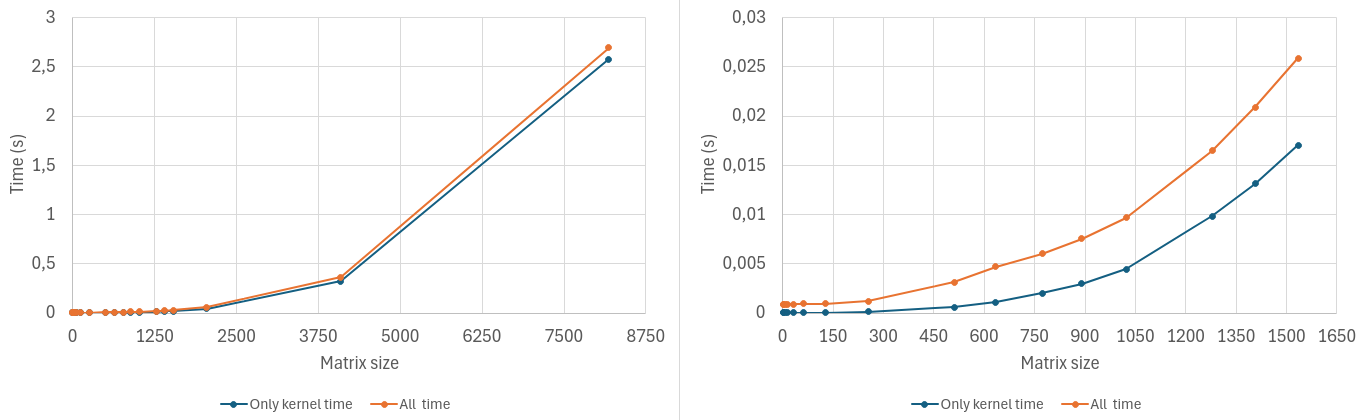
\includegraphics[width=0.85\textwidth]{img/4.png}
    \caption{Sólo el tiempo de ejecución del \textit{kernel} vs el tiempo total}
    \label{fig:4}
\end{figure}

Sorprendentemente, el tiempo de reserva de memoria y copia de resultados está muy optimizado ya que, con los tamaños de 
matriz probados, no hay apenas diferencia entre únicamente el tiempo de ejecución del \textit{kernel} y el tiempo total.
Aun así, si se probase con matrices de mucho mayor tamaño (poco funcional para esta práctica) seguramente la diferencia
sería notable.
